\documentclass[border=10pt]{standalone}

\usepackage[utf8]{inputenc}                                 % Codificação do documento
\usepackage[T1]{fontenc}                                    % Seleção de código de fonte
\usepackage{microtype}                                      % Melhora a justificação do documento
\usepackage{lmodern}                                       % Usa a fonte Latin Modern
\usepackage{ae, aecompl}                                    % Fontes de alta qualidade

\usepackage{amsmath}
\usepackage{verbatim}
\usepackage{tikz}
\usetikzlibrary{arrows,calc,positioning,shadows.blur,decorations.pathreplacing}
\usepackage{etoolbox}

\begin{document}
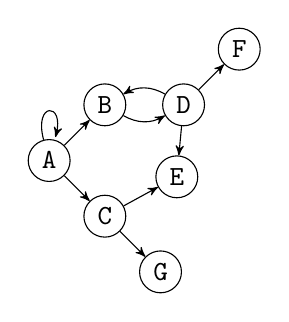
\begin{tikzpicture}
[
	              y = -1cm,
	           ->, >= stealth',
	  node distance = 2cm,
	  vertex/.style = { draw=black, circle, inner sep=2.5pt }
]
	% nodes
	\node (A) at (0,1)            [vertex]   {\texttt{A}};

	\node (B) at (0.7071,0.2929)  [vertex]   {\texttt{B}};
	\node (D) at (1.7071,0.2929)  [vertex]   {\texttt{D}};
	\node (E) at (1.6213,1.2071)  [vertex]   {\texttt{E}};
	\node (F) at (2.4142,-0.4142) [vertex]   {\texttt{F}};

	\node (C) at (0.7071,1.7071)  [vertex]   {\texttt{C}};
	\node (G) at (1.4142,2.4142)  [vertex]   {\texttt{G}};

	% edges
	\draw [->] (A) edge [loop above] (A);
	\draw [->] (A) edge (C) (C) edge (E) (C) edge (G);
	\draw [->] (A) edge (B) (B) edge [bend right] (D) (D) edge [bend right] (B) (D) edge (E) (D) edge (F);

\end{tikzpicture}
\end{document}